\section{Metrics for Performance Evaluation}
Metrics for performance evaluation focuses on the predictive capability of a model, that is, how well a model can predict the class of the test data, and evaluate the performance of the training-data.
Speed and scalability is not discussed in this section.

\subsection{Confusion Matrix}
One of the most common ways of doing this is through the confusion matrix:

\bigskip
\begin{figure}[H]
    \centering
    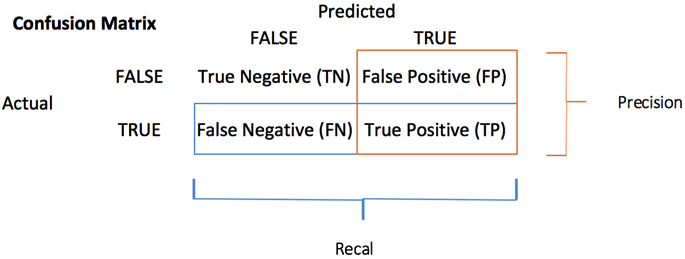
\includegraphics[scale=0.5]{figures/confusionmatrix.png}
    \caption{Confusion Matrix}
\end{figure}

The confusion matrix in this example has one axis for the true classes 
and one axis for the predicted classes. A correct classification is 
therefore on the diagonal. From this confusion almost all other metrics 
used in classification can be derived. A confusion matrix can also contain 
more than two classes. $TP$, $TN$, $FP$ and $FN$ is in those cases calculated
with respect to each class. One of the most common and 
widely-used metric for evaluating the performance is accuracy:

\begin{theo}[]{theo:theo500}
    \label{eq:accuracy}
        \[
            Accuracy = \frac{TP + TN}{TP + TN + FP + FN}
        \]
\end{theo}

The accuracy metric has some limitations, among those are the ability to evaluate two-class problems where almost all instances are of class 0, while only a few are of class 1.
The accuracy metric will result in $99.9\%$ accuracy, which is misleading if the model predicts all instances to belong to class 0.
Accuracy can also be calculated for each individual class where one calculates
$TP$, $TN$, $FP$ and $FN$ for the respected class as positive 
against all other classes considered negative. This may help combat some of
the limitations from using overall accuracy.

\subsection{Cost Matrix}

One way of solving the issue is to use a cost matrix instead:

\bigskip
\begin{figure}[H]
    \centering
    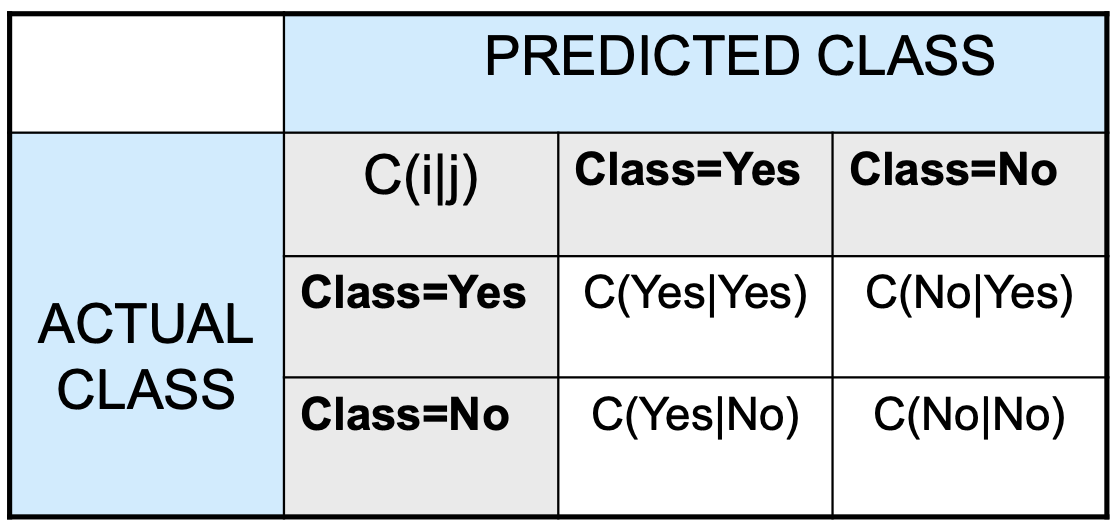
\includegraphics[scale=0.5]{figures/costmatrix.png}
    \caption{Cost Matrix}
\end{figure}

Here, $C(i|j)$ is the cost of misclassifying class $j$ as class $i$. The cost equals the weighted sum of all predictions.

\bigskip

If true positives and true negatives are equally weighted, as well as the fasle positives and the false negatives, the accuracy is proportional to the cost.
This results in the following equation:

\begin{equation}
    Cost = N[q-(q-p)*Accuracy]
\end{equation}
\begin{center}
    Where $N = TP + TN + FP + FN$, $q = FP$, and $p = TP$.
\end{center}


\subsection{Cost-Sensitive Measures}
Some cost-sensitive measures that are preferred over accuracy:

\begin{equation}
    \text{Precision}(p) = \frac{TP}{TP+FP}
\end{equation}

\begin{equation}
    \text{Recall}(r) = \frac{TP}{TP+FN}
\end{equation}

\begin{equation}
    \text{F-measure}(F) = \frac{2TP}{2TP+FP+FN}
\end{equation}

\begin{itemize}
    \item Precision is biased towards $TP$ and $FP$
    \item Recall is biased towards $TP$ and $FN$
    \item F-measure is biased towards all except $TN$
\end{itemize}

\begin{equation}
    \text{Weighted Accuracy} = \frac{\omega_1 TP + \omega_4 TN}{\omega_1 TP + \omega_2 FN + \omega_3 FP + \omega_2 TN}
\end{equation}

\section{Methods for Performance Evaluation}
Methods on how to obtain a reliable estimate of performance.

The performance of a model may depend on other factors besides the learning algorithm:
\begin{itemize}
    \item Class distribution.
    \item Cost of misclassification.
    \item Size of training and test sets.
\end{itemize}

\subsection{Learning Curve}
Learning curves show how accuracy changes with varying sample sizes.

Learning curves require a sampling schedule:
\begin{itemize}
    \item Arithmetic sampling. (Linear)
    \item Geometric sampling. (Exponential)
\end{itemize}

\bigskip
\begin{figure}[H]
    \centering
    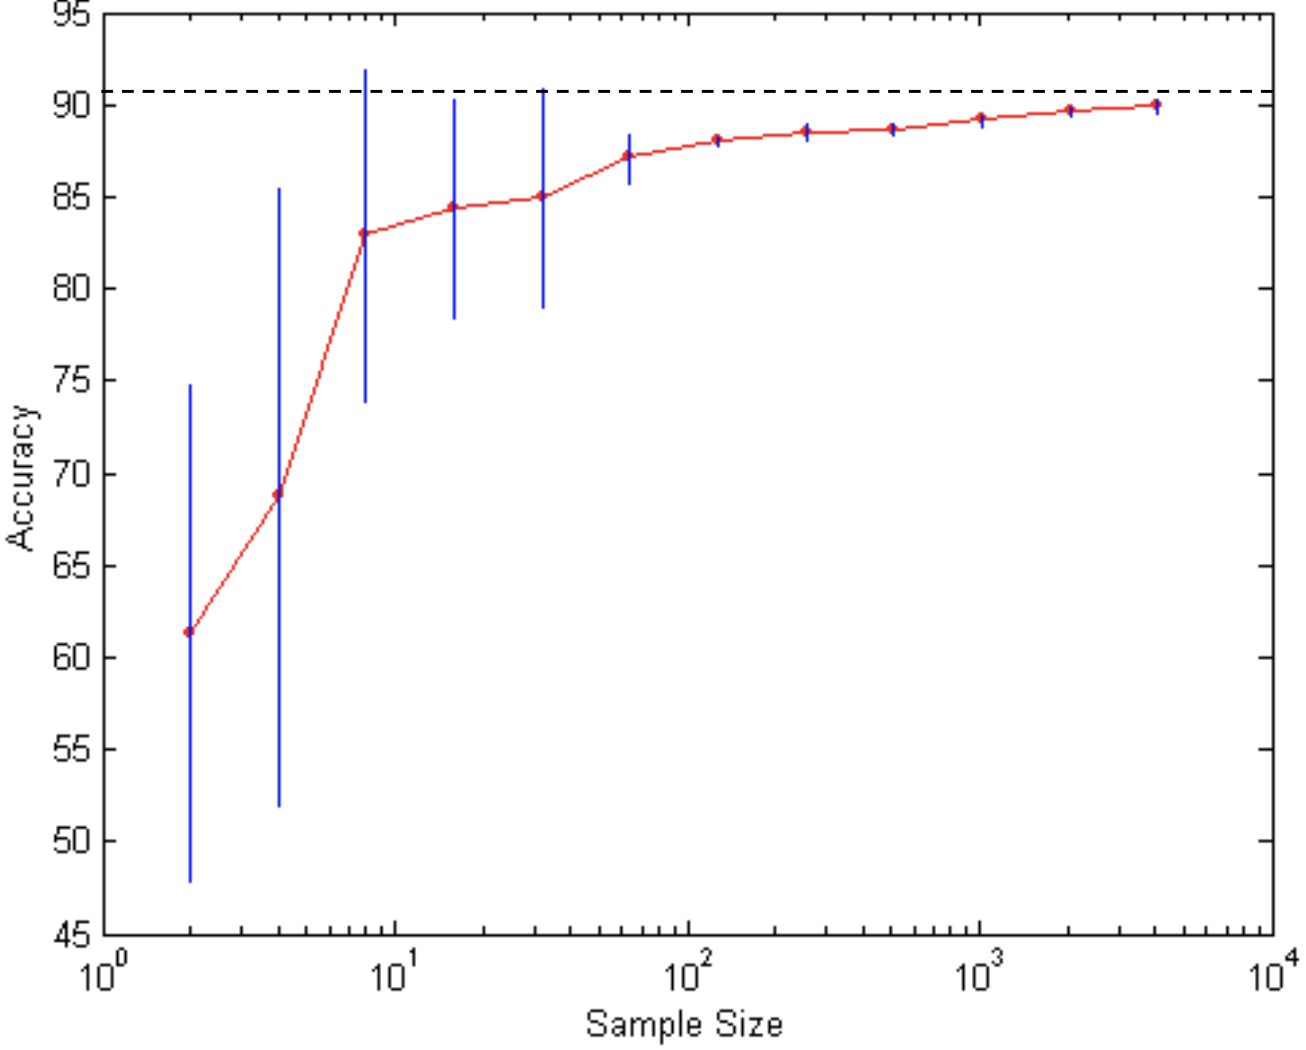
\includegraphics[scale=0.5]{figures/learningcurve.png}
    \caption{A Learning Curve}
\end{figure}

The effects of small sample sizes includes:
\begin{itemize}
    \item Bias in the estimate (Underfitting)
    \item Variance of estimate (Overfitting)
\end{itemize}

\subsection{Other Methods of Estimation}
\begin{itemize}
    \item Holdout
    \begin{itemize}
        \item Reserve $80\%$ for training and $20\%$ for testing.
    \end{itemize}
    \item Random subsampling
    \begin{itemize}
        \item Repeated holdouts
    \end{itemize}
    \item Cross validation (popular)
    \begin{itemize}
        \item Partition data into $k$ disjoint subsets.
        \item $k$-fold: Train on $k-1$ partitions, test on the remaining one.
        \item Leave-one-out: $k=n$
    \end{itemize}
    \item Stratified sampling
    \begin{itemize}
        \item Oversampling
        \item Undersampling
    \end{itemize}
    \item Bootstrap
    \begin{itemize}
        \item Sampling with replacement
    \end{itemize}
\end{itemize}

\newpage
\section{Methods for Model Comparison}
Methods for model comparison explains how to compare the relative performance among competing models.

\subsection{Receiver Operating Characteristic (ROC)}
ROC was developed in the 1950s to characterize the trade-off between true positives and false positives.

A ROC curve plots $TP$ on the $y$-axis against $FP$ on the $x$-axis, where the performance of each classifier is represented as a point on the ROC curve.
The point changes based on the threshold of the algorithm, the sample distribution, and/or the cost matrix.

\bigskip
\begin{figure}[H]
    \centering
    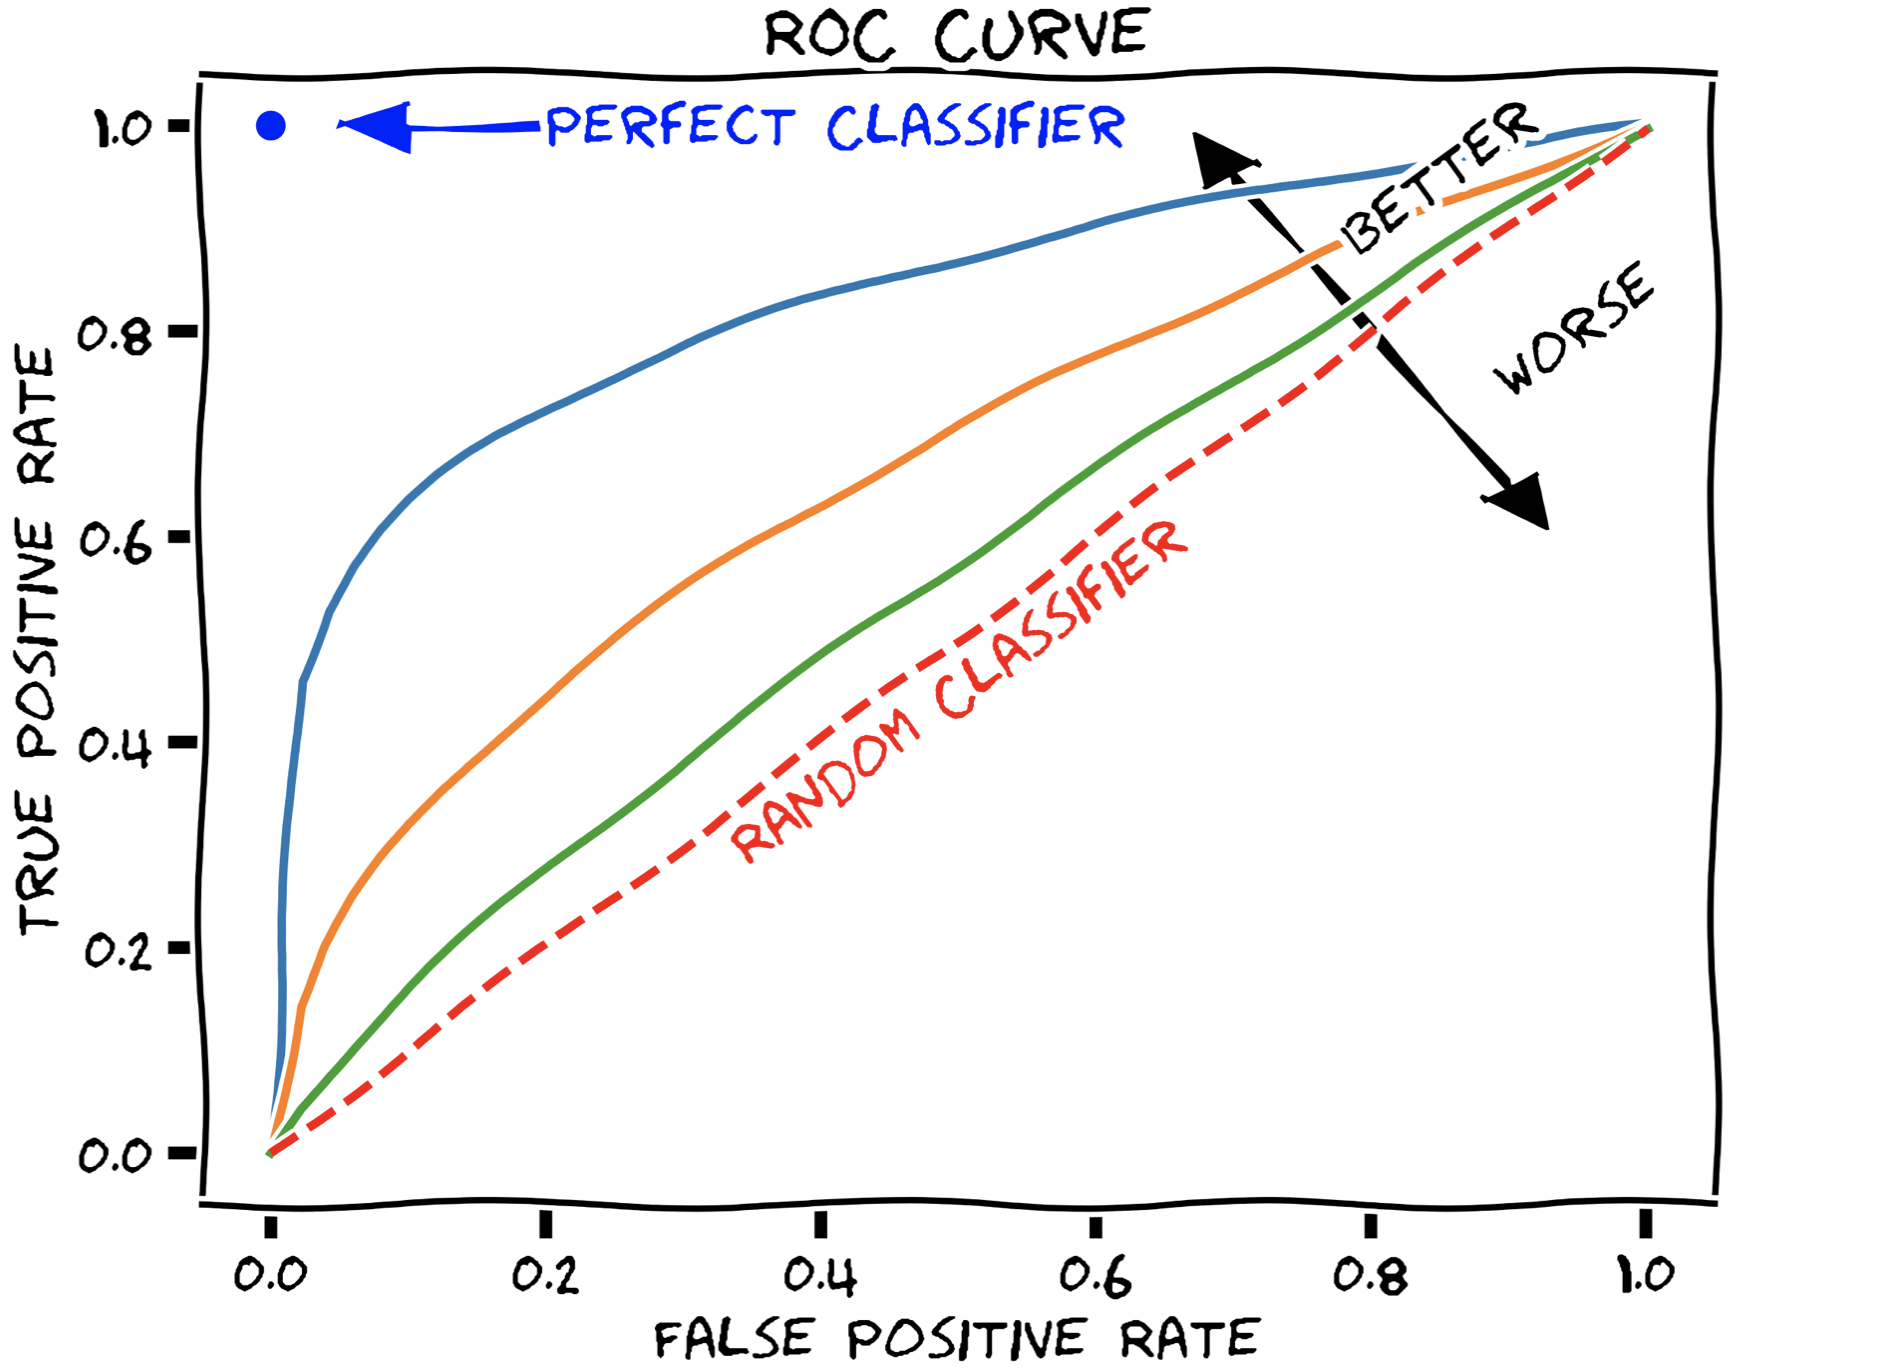
\includegraphics[scale=0.25]{figures/roccurve.png}
    \caption{ROC Curve}
\end{figure}

In some cases when comparing the ROC curve for different models, no models consistently outperform the others. Evaluating such models can be based on the area under the ROC curve (AUC), or which model fits better to the desired outcome.

\subsubsection{Constructing a ROC curve}
\begin{enumerate}
    \item Use a classifier that produces posterior probability for each test instance $P(+|A)$.
    \item Sor the instances according to $P(+|A)$ in decending order.
    \item Apply threshold at each unique value of $P(+|A)$.
    \item Count the number of $TP$, $FP$, $TN$ and $FN$ at each treshold.
\end{enumerate}
\begin{itemize}
    \item $TPR = \frac{TP}{TP+FN}$
    \item $FPR = \frac{FP}{FP+TN}$
\end{itemize}
